\documentclass[tikz,border=10pt]{standalone}
\usepackage{tikz}
\usetikzlibrary{calc}
\begin{document}
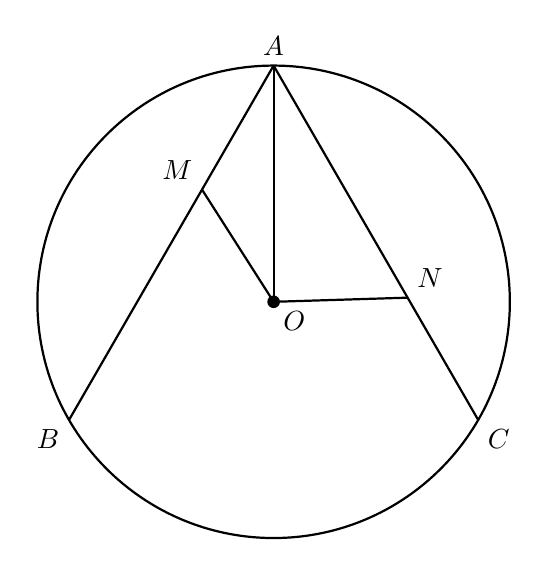
\begin{tikzpicture}[scale=2]
  % Draw the circle
  \draw[thick] (0,0) circle (1.5);
  
  % Define points on the circle
  \coordinate (A) at (0,1.5);
  \coordinate (B) at (-1.299,-0.75);
  \coordinate (C) at (1.299,-0.75);
  
  % Define center point
  \coordinate (O) at (0,0);
  
  % Define points M and N on the circle
  \coordinate (M) at ($(A)!0.35!(B)$);
  \coordinate (N) at ($(A)!0.655!(C)$);
  
  % Draw lines connecting points
  \draw[thick] (A) -- (B);
  \draw[thick] (C) -- (A);
  \draw[thick] (A) -- (O);
  \draw[thick] (M) -- (O);
  \draw[thick] (N) -- (O);
  \fill (O) circle (0.04);
  % Label the points
  \node[above] at (A) {$A$};
  \node[below left] at (B) {$B$};
  \node[below right] at (C) {$C$};
  \node[below right] at (O) {$O$};
  \node[above left] at (M) {$M$};
  \node[above right] at (N) {$N$};
\end{tikzpicture}
\end{document}